\chapter{Dataset}\label{chap:dataset}

In this chapter, we describe the data and discuss how we filter reviews to get more reliable data with less noise.
Next, we describe what features we extracted
and report statistics about the dataset and features.

\section{Format of the Dataset}\label{sec:format}

Yelp is a US-based company whose goal is: ``to connect people with great local businesses.''\footnote{\url{https://yelp.com/about}}
It provides both mobile and web interface listing businesses such as restaurants or shopping centres.
Users can easily post a review for any business based on their recent visit.
Its convenience and usefulness makes the platform very popular.

It works in a similar manner like other recommendation systems such as IMDB\footnote{Internet Movie Database \url{https://www.imdb.com/}} or
TripAdvisor.\footnote{\url{https://www.tripadvisor.com}}
There are restaurant profiles to which users can add reviews.
Users can search for restaurants based on various parameters as shown in \Cref{fig:filters}.

\begin{figure}[ht]\centering
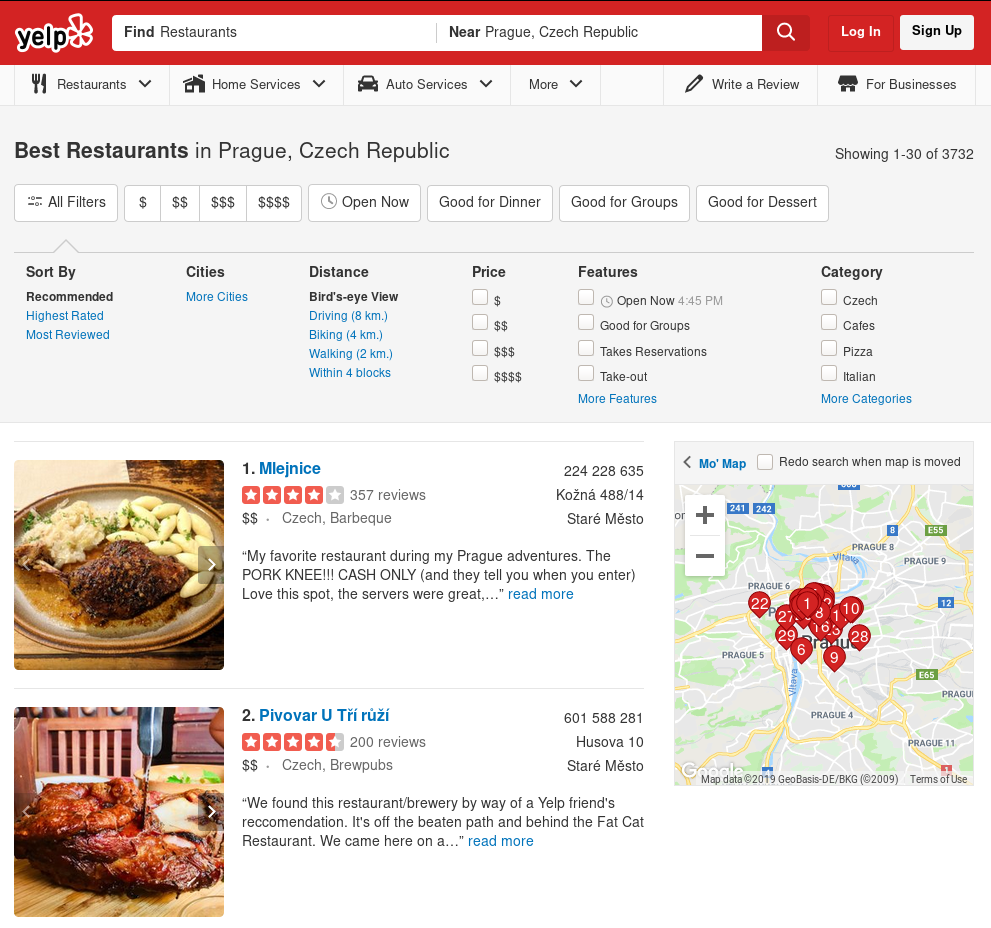
\includegraphics[width=130mm]{../img/filters.png}
\caption{Seeking restaurants with parameters}
\label{fig:filters}
\end{figure}

An example of a profile is shown in \Cref{fig:dobra_trafika_app}.
On the sides, various information such as price range or opening time is shown.
The main part is devoted to reviews.
Every review clearly displays the number of stars awarded and the text.
Also, Yelp already works with some sort of usefulness,
because two reviews have been hidden as can be seen in the bottom of the picture.

Yelp also allows users to flag properties of other reviews in the form of \emph{likes}.
Each review has three buttons --- \emph{useful}, \emph{funny} and \emph{cool} as can be seen in \Cref{fig:dobra_trafika_app}.
A user can vote for the property of a review by clicking on one of these buttons.

\begin{figure}[ht]\centering
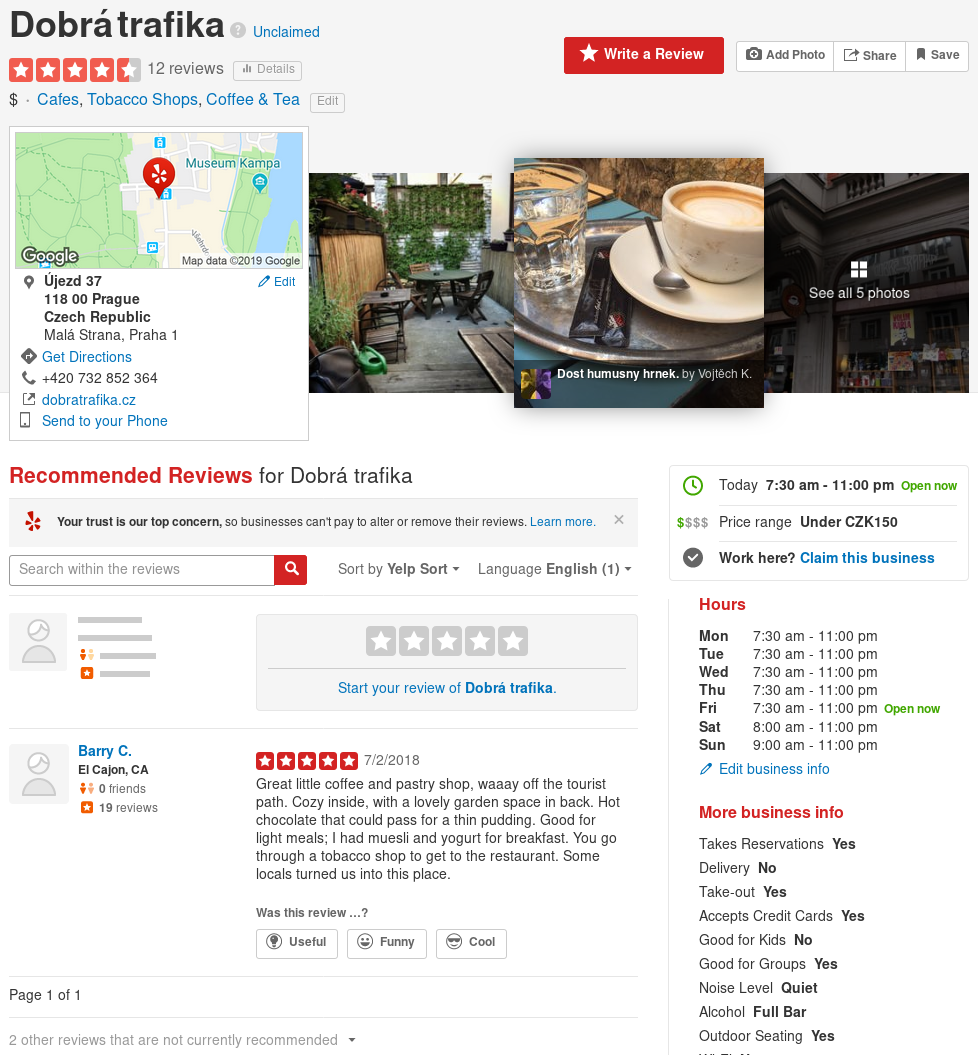
\includegraphics[width=130mm]{../img/dobra_trafika.png}
\caption{An example of an online profile}
\label{fig:dobra_trafika_app}
\end{figure}

There are three main reasons we chose Yelp reviews: 

\begin{itemize}
\item this platform is very popular and as such has sufficient data.

\item the company publishes every year an open dataset which can be downloaded for academic
purposes.
It covers most information conveyed in their system ---  information about businesses and users, pictures taken by the users and textual reviews.
The data is available for download and we can focus on building our programme, rather than obtaining data.

\item  the dataset contains the information how many times the like buttons have been clicked on.
This allows us to asses the needed properties of individual reviews and
we use it to distinguish useful and not-useful reviews.
\end{itemize}


We use files \texttt{review.json} and \texttt{business.json} from the dataset.
The former contains reviews represented by JSON.
There is one review per line.\footnote{In fact, it is JSON lines format --- \url{https://jsonlines.org}}

Every review contains unique ID and business ID which is a reference to a business in file \texttt{business.json}.
It also contains data about the review itself; review text, date of publishing and number of individual likes it received so far.
Also, every review is accompanied by a star rating.
The interval is one to five stars; five being the best.
An example of a prettified review is in \Cref{fig:review}.

\begin{figure}[t]\centering
\begin{code}
{
	"review_id": "---nya_pjxWmNFDFyAcfsA",
	"user_id": "5QOtcHU1SoqEqBCRR6FhsA",
	"business_id": "zQNJwaWR1M1zDjLNVJiNEw",
	"stars": 1,
	"date": "2012-06-27",
	"text": "Another case of the Emperor's New Clothes...",
	"useful": 10,
	"funny": 2,
	"cool": 3
}
\end{code}
\caption{An example of a review in JSON}\label{fig:review}
\end{figure}

The second file we use is \texttt{business.json}.
Again, it is in JSON lines and it contains business information such as opening hours or availability of a car park.
An example of a business can be found in \Cref{fig:business}.

\begin{figure}[t]\centering
\begin{code}
{
	"business_id": "zQNJwaWR1M1zDjLNVJiNEw",
	"name": "Pizza M",
	"neighborhood": "",
	"address": "208 W Main St",
	"city": "Urbana",
	"state": "IL",
	"postal_code": "61801",
	"latitude": 40.112655,
	"longitude": -88.2093142,
	"stars": 3.5,
	"review_count": 60,
	"is_open": 1,
	"attributes": {
		"RestaurantsTableService": false,
		"Alcohol": "beer_and_wine",
		"Caters": false,
		"HasTV": false,
		"RestaurantsGoodForGroups": true,
		"NoiseLevel": "average",
		"WiFi": "free",
		"RestaurantsAttire": "casual",
		"RestaurantsReservations": false,
		"OutdoorSeating": false,
		"BusinessAcceptsCreditCards": true,
		"RestaurantsPriceRange2": 2,
		"BikeParking": true,
		"RestaurantsDelivery": true,
		"RestaurantsTakeOut": true,
		"GoodForKids": true,
		"BusinessParking": {
			"garage": true,
			"street": true,
			"validated": false,
			"lot": false,
			"valet": false
		}
	},
	"categories": ["Restaurants", "Pizza"],
	"hours": {
		"Monday": "11:00-21:00",
		"Tuesday": "11:00-21:00",
		"Friday": "11:00-22:00",
		"Wednesday": "11:00-22:00",
		"Thursday": "11:00-22:00",
		"Sunday": "11:00-21:00",
		"Saturday": "11:00-23:00"
	}
}
\end{code}
\caption{An example of a business}\label{fig:business}
\end{figure}

There are other files that could contain potentially useful information.
File \texttt{user.json} is possibly interesting, because it contains information about users.
There is a cross reference from reviews to users in the same manner as businesses,
so we could get potentially useful information for every review;
for example the number of reviews already posted by the author or
how long the poster has been registered on Yelp.

We decided not to use this file for three main reasons.
First, the data is very sparse and it would be hard to avoid overfitting or gain significant improvement.
Second, There is a lot of information about users resulting in very big denormalized data
and as such hard to work with.
Lastly and most importantly, this thesis focuses on extracting information from text rather than from metadata.

For easier manipulation, we denormalized the data.
We also added the information from a spellchecker.\footnote{\url{https://aspell.net}}
Every review was added the information of number of words and number of misspelled words to the review.
These two values were used for feature extraction.

The resulting data has been saved in an instance file,
which is in JSON lines containing an instance per line.
An instance is a review with the element \texttt{business\_id} replaced by the business information.
An example of a full instance is in \Cref{fig:full_instance}.

\begin{figure}[t]\centering
	\begin{codetiny}
{
	"review_id": "---nya_pjxWmNFDFyAcfsA",
	"user_id": "5QOtcHU1SoqEqBCRR6FhsA",
	"business_id": {
		"business_id": "zQNJwaWR1M1zDjLNVJiNEw",
		"name": "Pizza M",
		"neighborhood": "",
		"address": "208 W Main St",
		"city": "Urbana",
		"state": "IL",
		"postal_code": "61801",
		"latitude": 40.112655,
		"longitude": -88.2093142,
		"stars": 3.5,
		"review_count": 60,
		"is_open": 1,
		"attributes": {
			"RestaurantsTableService": false,
			"Alcohol": "beer_and_wine",
			"Caters": false,
			"HasTV": false,
			"RestaurantsGoodForGroups": true,
			"NoiseLevel": "average",
			"WiFi": "free",
			"RestaurantsAttire": "casual",
			"RestaurantsReservations": false,
			"OutdoorSeating": false,
			"BusinessAcceptsCreditCards": true,
			"RestaurantsPriceRange2": 2,
			"BikeParking": true,
			"RestaurantsDelivery": true,
			"RestaurantsTakeOut": true,
			"GoodForKids": true,
			"BusinessParking": {
				"garage": true,
				"street": true,
				"validated": false,
				"lot": false,
				"valet": false
			}
		},
		"categories": ["Restaurants", "Pizza"],
		"hours": {
			"Monday": "11:00-21:00",
			"Tuesday": "11:00-21:00",
			"Friday": "11:00-22:00",
			"Wednesday": "11:00-22:00",
			"Thursday": "11:00-22:00",
			"Sunday": "11:00-21:00",
			"Saturday": "11:00-23:00"
		}
	},
	"stars": 1,
	"date": "2012-06-27",
	"text": "Another case of the Emperor's New Clothes...",
	"useful": 10,
	"funny": 2,
	"cool": 3,
	"words": 57,
	"incorrect_words": 0
}
\end{codetiny}
\caption{An example of a full instance}\label{fig:full_instance}
\end{figure}



\section{Filtering Reviews}\label{sec:filter}


The number of likes is a problematic metric for usefulness.
Different reviews having the same ``level'' of usefulness can vary greatly
in the number of likes.
One of the biggest influences is the age of reviews and online popularity.
Also, the social group visiting the business has a considerable impact.
Locals going to the same pub for years will not produce nearly as much traffic
as a touristic spot.
Reviews for a club for young people will have different rates of visits and likes
than a place for families.

Using all reviews directly would therefore be problematic.
We tried to reduce the variance by filtering out reviews.
We use only reviews belonging to businesses with \textbf{at least 50 reviews and 10 attributes}.
By attributes, we mean the restaurants attributes such as opening hours and Wi-Fi availability.
This condition omits infrequently visited restaurants where the number of likes could fluctuate a lot.
Also, it avoids restaurants with incomplete online profile which may be less likely to be reviewed.

To avoid the problem with age, we used only reviews posted in a very specific date frame
--- \textbf{between 1$^{st}$ May 2012 and 1$^{st}$ December 2012}.
Thanks to this all reviews have been exposed for the same time to receive likes.

Note that the dataset contains general businesses, but we focus on restaurants only.
When we analysed filtered reviews,
there were less than 30,000 reviews for non-restaurants out of total 206,000.
Because the rate is rather small,
we decided to treat all businesses the same way as restaurants.

Because we focus on English only, we filter out French and German.
Other languages have been left intact, because they presence is not significant.

For language recognition, we used very simple approach.
We used the ratio of incorrect words to detect language.
We computed the ratio of misspelled and correct words for English, German and French and
picked the language with the lowest ratio.
This approach is not perfect the spell checker's dictionary does not cover all words, or a misspelled word may be incidentally another word.
However, It worked surprisingly well, even though many English words such as ``credit card'' or ``hamburger'' are used in the other languages too.

We also decided to drop reviews with exactly one useful like.
One like may only be an accident such as an unintentional click or some other noise.

In short, we used only reviews satisfying all of the following:

\begin{itemize}
	\item the corresponding restaurant has at least at least 50 reviews and 10 attributes
	\item posted between 1$^{st}$ May 2012 and 1$^{st}$ December 2012
	\item not in French or German
	\item zero or at least two useful likes
\end{itemize}

The filtering produces dataset containing 64,550 instances.
The resulting dataset was labelled according to the number of useful likes.
Reviews with zero likes were labelled not-useful and
reviews with at least two likes useful.
The entire dataset contains 44,921 not-useful and
19,629 useful instances.



\section{Data Statistics}\label{sec:data_stats}

In this section, we define features
and report basic statistics conducted on the entire final dataset.

We split features into the sets defined in the two lists bellow;
\textbf{phrase features} expressing whether certain phrase is present in the review and
\textbf{threshold features} clustering reviews into groups.
Most of the features are binary with exceptions noted in the feature descriptions.

Note that the best way for selecting bigrams and trigrams would be to compute mutual information of all bigrams, resp. trigrams.
However, this is computationally very expensive, as there are well over 1,100,000 unique bigrams in the reviews.
Instead, we decided to use n-grams that consist of only top informative unigrams.

\subsubsection*{Phrase features}

\begin{itemize}
	\item UNIGRAMS --- top 50,000 unigrams according to mutual information
	\item BIGRAMS --- bigrams consisting of top 25,000 adjacent unigrams
	\item TRIGRAMS  --- trigrams consisting of top 10,000 adjacent unigrams
	\item TFIDF  --- top 50,000 words
	\item ENTITIES --- 270,000 entities as found by the NLP analysis
\end{itemize}

\subsubsection*{Threshold features}

\begin{itemize}
	\item STARS 
		\begin{itemize}
			\item the number of stars; five binary features
			\item indicators for each stars number; five binary features one-vs-rest
			\item extreme stars; binary with one group 1 or 5 stars; the rest another group
			\item the number of average stars for the business; five groups
		\end{itemize}
	\item REVIEWLEN 
		\begin{itemize}
			\item the number of words; ternary with thresholds 50 and 150
			\item the number of words; five binary features with thresholds 35, 50, 75, 100 and 150
		\end{itemize}
	\item SPELLCHECK 
		\begin{itemize}
			\item the rate of misspelled words; five binary features with thresholds 0.02, 0.05, 0.1, 0.15 and 0.2
			\item the number of misspelled words; four binary with thresholds 5, 10, 15 and 20
		\end{itemize}
	
	\item COSINESIM --- cosine similarity to 10 randomly chosen useful instances; five binary features with thresholds 0.4, 0.6, 0.8, 0.9, 0.95
\end{itemize}

The average number of words in a review is 151 and the number distribution can be seen
in \Cref{fig:word_hist}.
From the cropped histogram in \Cref{fig:word_hist_crop}, we can see that all our features
referring to the number of words split the dataset into two or three non-empty groups.

\begin{figure}[ht]\centering
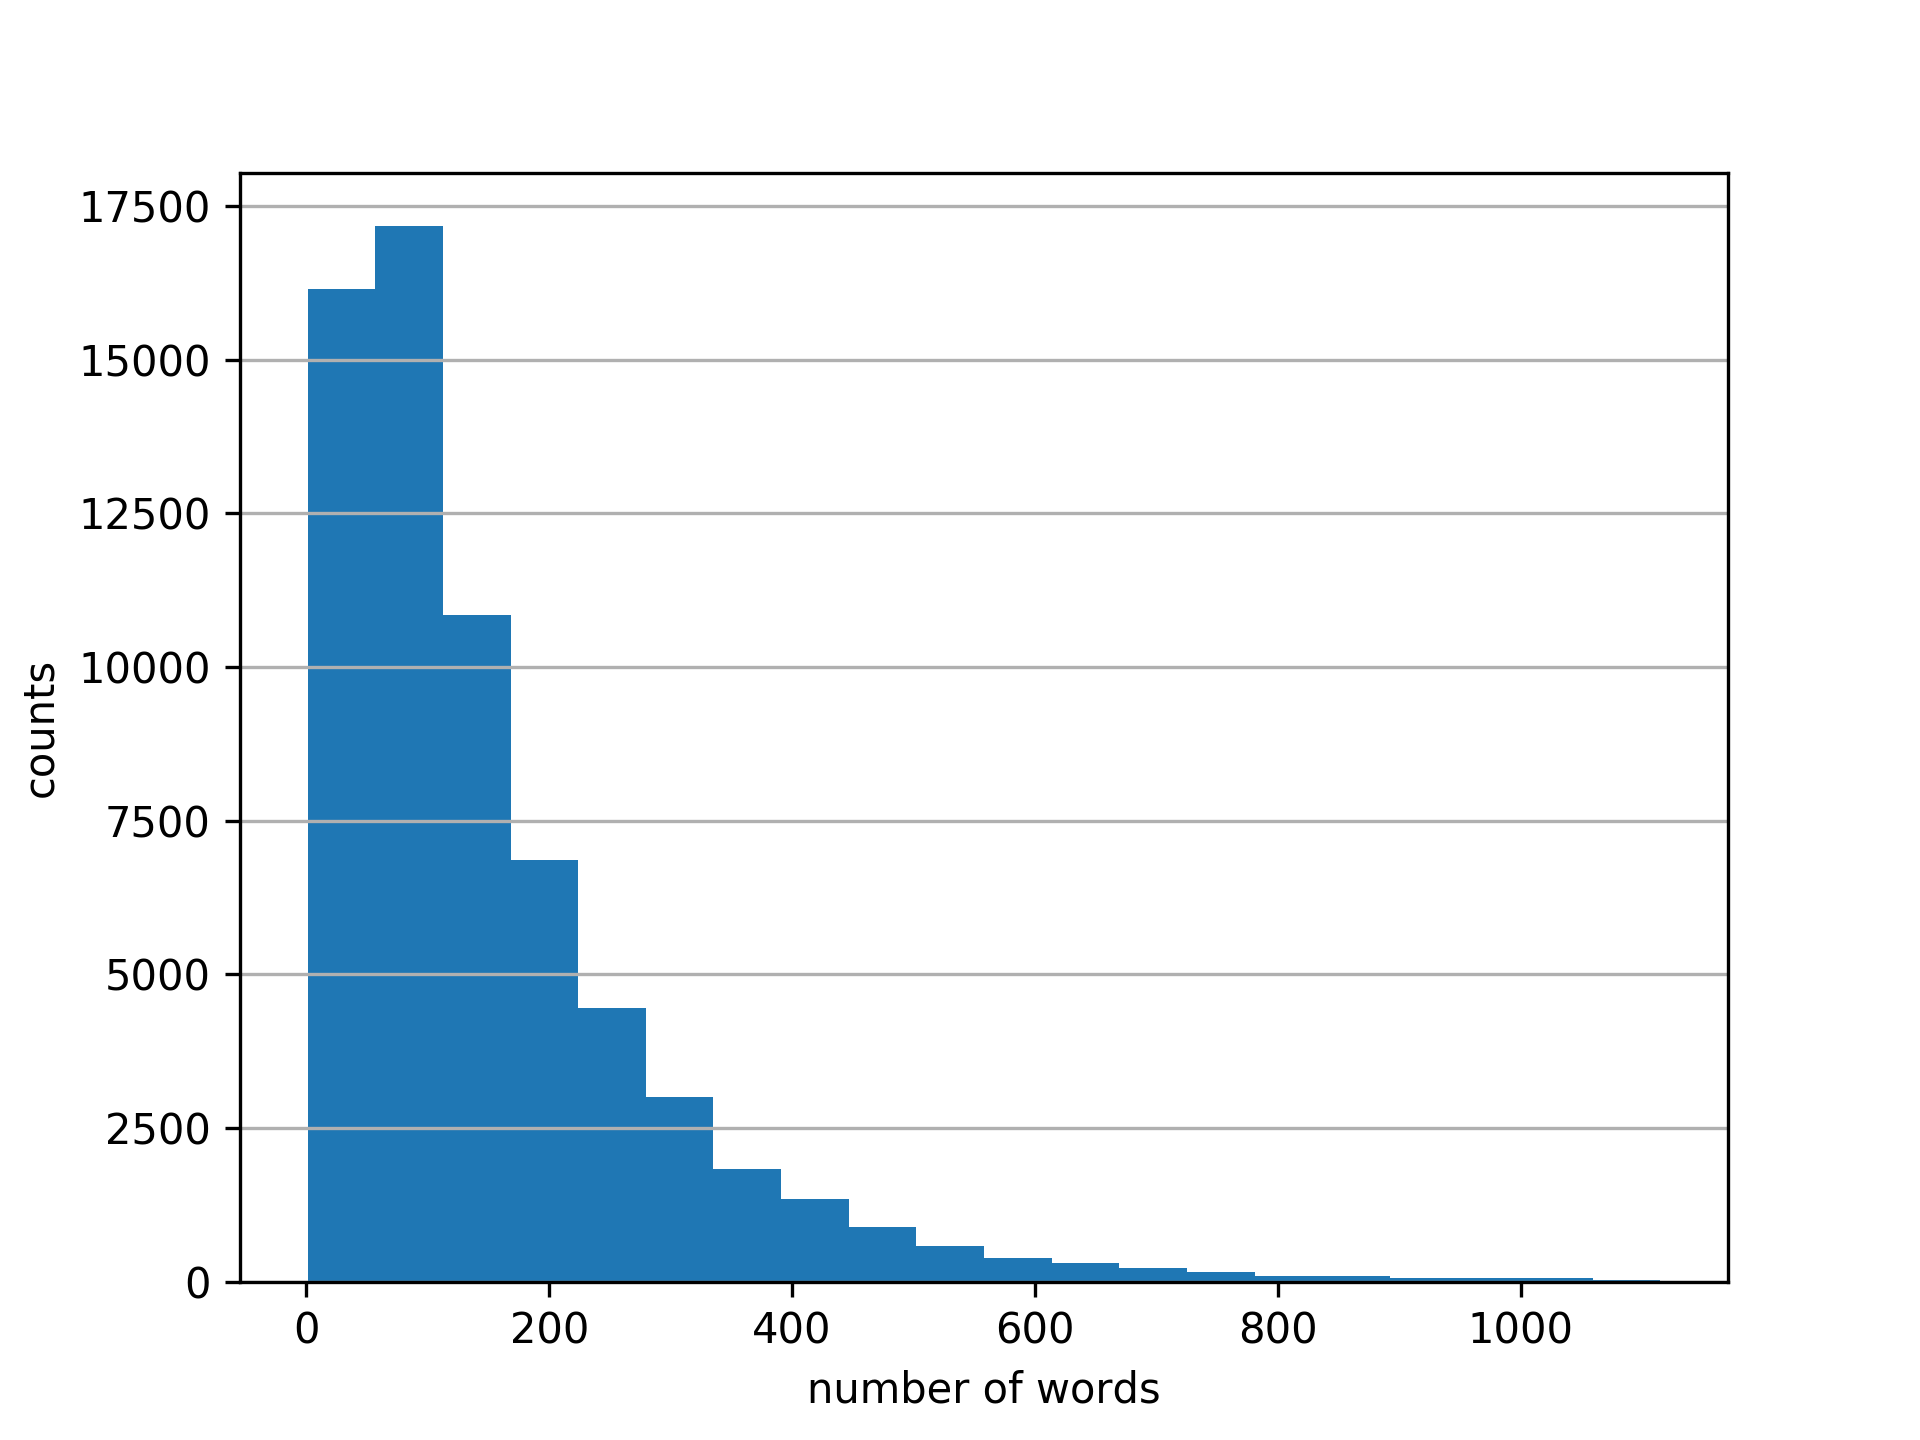
\includegraphics[width=130mm]{figures/word_hist.png}
\caption{Histogram of number of words in reviews}\label{fig:word_hist}
\end{figure}

\begin{figure}[ht]\centering
	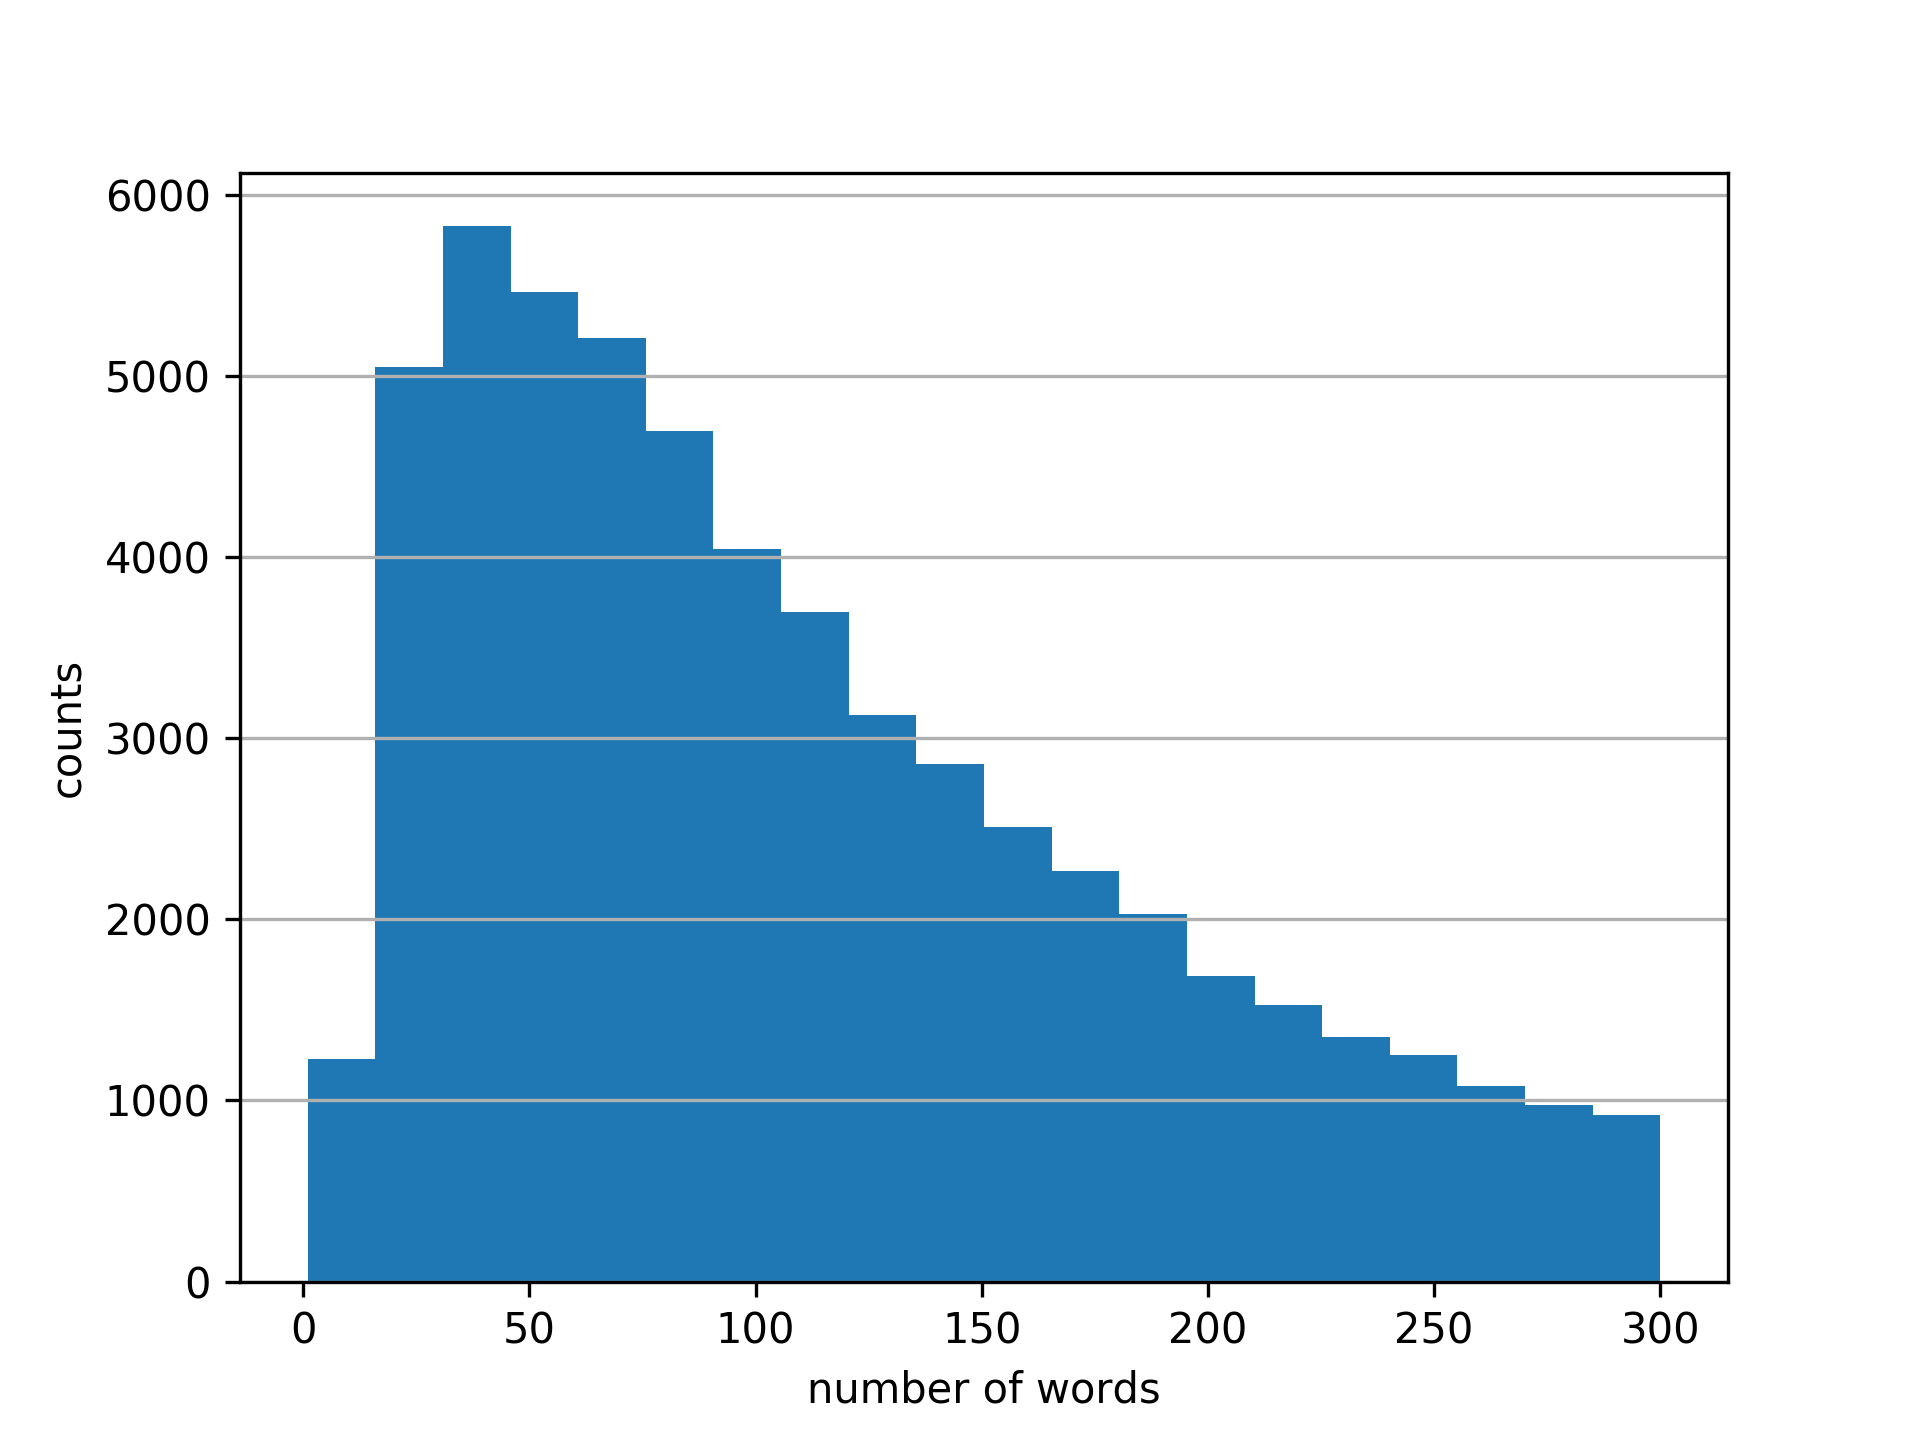
\includegraphics[width=130mm]{figures/word_hist_cropped.png}
\caption{Words histogram zoomed in for up to 300 words}\label{fig:word_hist_crop}
\end{figure}


The average number of phrases contained in a review can be seen in \Cref{tab:phrase_feat_nu}.
It is worth noting that the average number of single words chosen by tf-idf and by mutual information is virtually the same.

The average number of entities is significantly lower than the number of bigrams or trigrams.
This is likely because the entities are chosen such that they actually mean something,
whereas bigrams are chosen whenever they consist of informative unigrams.
\begin{table}[h!]
\centering
\begin{tabular}{lr@{~}r@{~}r@{~}r}
\toprule
\textbf{name}	& \multicolumn{4}{c}{\textbf{average number}} \\
\midrule
tf-idf  & 89 & (1, 481) & $\pm$& 63 \\
unigrams & 89 & (1, 482) & $\pm$& 63 \\
bigrams & 135 & (0, 942) & $\pm$ &120 \\
trigrams & 134 & (0, 1012) & $\pm$& 124 \\
entities & 16 & (0, 144) & $\pm$ &13 \\
\bottomrule
\end{tabular}


\caption{Number of phrase features}\label{tab:phrase_feat_nu}
All reported values are in the format ` arithmetic mean (min, max) $\pm$ standard deviation'.
\end{table}


Distribution of discrete features is reported in \Cref{tab:star_distr}.
We can that stars shifted to higher numbers, most reviews giving
four or five stars.
This is in accordance with sentiment, which has by far the most positive reviews.
Reviews for which sentiment could not be computed are labeled \texttt{n/a}.

Stars given to the particular business also have the average 3.7.
However, very few businesses have 4.5 or 5 stars.

Error rate splits reviews into different clusters, only thresholds 0.02 and 0.05
having both clusters with significantly many reviews.
On the other hand, the number of total errors was always bellow the threshold and 
thus bringing literary no information.

\begin{table}[h!]
\centering
\begin{tabular}{llr}
\toprule
\textbf{name} & \textbf{property} & \textbf{value} \\
\midrule
stars 	& average	& 3.7 \\
		&1			& 5413 \\
		& 2			& 6508 \\
		& 3			& 10453 \\
		& 4			& 21912 \\
		& 5			& 20264 \\
\midrule
sentiment & n/a & 30 \\
&   negative & 4365 \\
&   neutral & 19194 \\
&   positive & 40961 \\
\midrule
error rate & $\le$ 0.02 & 30572 \\
		   & $>$ 0.02 & 33979 \\
\midrule
		   & $\le$ 0.05 & 8740 \\
		   & $>$ 0.05  & 55810 \\
\midrule
		   & $\le$ 0.1 & 1551 \\
		   & $>$ 0.1  & 63099 \\
\midrule
		   & $\le$ 0.15 & 453 \\
		   & $>$ 0.15  & 64197 \\
\midrule
		   & $\le$ 0.2 & 191 \\
		   & $>$ 0.2  & 64359 \\
\midrule
error total & $\le$ 5  & 64550 \\
			& $>$ 5 & 0 \\
\midrule
			& $\le$ 15  & 64550 \\ 
			& $>$ 15 & 0 \\
\midrule
			& $\le$ 20  & 64550 \\
			& $>$ 20 & 0 \\
\midrule
			& $\le$ 10  & 64550 \\
			& $>$ 10  & 0 \\
\midrule
business stars & average & 3.7 \\
 & 1.5 & 39 \\
 & 2.0 & 434 \\
 & 2.5 & 2346 \\
 & 3.0 & 8385 \\
 & 3.5 & 19871 \\
 & 4.0 & 26456 \\
 & 4.5 & 6962 \\
 & 5.0 & 61 \\
\bottomrule
\end{tabular}


\caption{Review stars distribution}\label{tab:star_distr}

\end{table}




\section{Mutual Information}\label{sec:mi}

After defining features, we report their mutual information (\textbf{MI} for short) with labels.
We use it for getting the idea of individual features and
to see if thresholds were chosen right.

Mutual information is a great way to evaluate informativeness of features.
However, it tends to prefer features of higher arity, because
they are more likely to decrease the entropy.
This can be observed in \Cref{tab:mi_words} and \Cref{tab:mi_stars}.


\subsection{Threshold Features}

First, we report MI of threshold features as listed in \Cref{chap:exp}.
Threshold features cluster instances into groups based on some numeric value.
In the tables bellow, there are features listed with different thresholds.
Thresholds correspond to values noted in the list in \Cref{sec:data_stats}.


In \Cref{tab:mi_errors}, we report MI of features regarding spelling mistakes.
Feature conveying absolute number of typos has negligible MI, probably owing to the high variance in the reviews' length.
On the contrary, the relative number of typos has proven to be an informative property.
The best performing having MI almost~0.002.

\begin{table}[h!]

\centering
\begin{tabular}{lrS[table-format=3.2]}
\toprule
\textbf{feature} & \textbf{threshold} & \textbf{mutual information} \\
\midrule
error rate & 0.02 & 0.00007 \\
\textbf{error rate} & 0.05 & 0.00182 \\
\textbf{error rate} & 0.10 & 0.00174 \\
error rate & 0.15 & 0.00074 \\
error rate & 0.20 & 0.00038 \\
\midrule
error total & 5 & 0.00000 \\
error total & 10 & 0.00000 \\
error total & 15 & 0.00000 \\
error total & 20 & 0.00000 \\
\bottomrule
\end{tabular}

\caption{Mutual information of spelling mistakes}\label{tab:mi_errors}
\end{table}


The features conveying the number of words turned out to be very informative.
The best performing was the feature with thresholds 50 and 150 having MI 0.07866 which
is more than 40 times more than the best performing error rate.

\begin{table}[h!]

\centering
\begin{tabular}{lrS[table-format=3.2]}
\toprule
\textbf{feature} & \textbf{threshold} & \textbf{mutual information} \\
\midrule
\textbf{review length} & 50, 150 & 0.07866 \\
review length & 35 & 0.02680 \\
review length & 50 & 0.04091 \\
review length & 75 & 0.05996 \\
review length & 100 & 0.06726 \\
review length & 150 & 0.06580 \\

\bottomrule
\end{tabular}
\caption{Mutual information of the number of words}\label{tab:mi_words}
\end{table}

Sentiment has MI approximately 0.01, which is about ten times higher
than error rate, but eight times worse than the number of words.

\begin{table}[h!]
\centering
\begin{tabular}{lrS[table-format=3.2]}
\toprule
\textbf{feature} & \textbf{threshold} & \textbf{mutual information} \\
\midrule
sentiment & neg, neut, pos & 0.00969 \\
\bottomrule
\end{tabular}
\caption{Mutual information of sentiment}\label{tab:mi_sentiment}
\end{table}

It follows from the experiments, that it greatly depends what instances
we choose for the cosine similarity features.
Only two out of ten instances in the cosine similarity corpus resulted in
non-negligible MI.
The best performing instances has MI of~\num{0.00006}, which is insignificant
in comparison with other features.

\begin{table}[h!]
\centering
\begin{tabular}{lrS[table-format=3.2]}
\toprule
\textbf{feature} & \textbf{threshold} & \textbf{mutual information} \\
\midrule
\textbf{instance 1} & 0.40 & 0.00006 \\
instance 1 & 0.60 & 0.00002 \\
instance 1 & 0.80 & 0.00002 \\
instance 1 & 0.90 & 0.00002 \\
instance 1 & 0.95 & 0.00002 \\
\midrule
\textbf{instance 2} & 0.40 & 0.00004 \\
instance 2 & 0.60 & 0.00002 \\
instance 2 & 0.80 & 0.00002 \\
instance 2 & 0.90 & 0.00002 \\
instance 2 & 0.95 & 0.00002 \\
\bottomrule
\end{tabular}
\caption{Mutual information of cosine similarity (2 best performing instances)}\label{tab:mi_cossim}
\end{table}

The best performing feature for stars convey the exact number of stars.
It has MI 0.01, which is comparable to sentiment.

The second best feature, \textit{whether the number of stars equals one}, shows a disadvantage of mutual information as a metrics for evaluate goodness of features.

The MI is fairly high and the feature looks useful at first.
Reviews giving only one star are likely to express serious complains, which are probably more useful than praising a business.
Data analysis backs this claim --- approximately 78\% of 1 star reviews have been repeatedly marked as useful.
However, the problem is that there is only as much as 0.4\% reviews giving 1 star making this
feature virtually worthless.

\begin{table}[h!]
\centering
\begin{tabular}{lrS[table-format=3.2]}
\toprule
\textbf{feature} & \textbf{threshold} & \textbf{mutual information} \\
\midrule
biz stars & 1, 2, 3, 4, 5 & 0.00112 \\
extreme stars & 1, 5 & 0.00175 \\
\textbf{stars} & 1, 2, 3, 4, 5& 0.01060 \\
stars & 1 & 0.00657 \\
stars & 2 & 0.00204 \\
stars & 3 & 0.00221 \\
stars & 4 & 0.00137 \\
stars & 5 & 0.00004 \\
\bottomrule
\end{tabular}

\caption{Mutual information of stars}\label{tab:mi_stars}
\end{table}


\subsection{Phrase Features}

Second, we report mutual information of phrase features.
Those features express whether a certain phrase exist in the text.

The value of the function in the two graphs bellow expresses
MI of the~$x$-th best feature at the point~$x$.
It is the same as if we ordered the feature in the descending order
and plotted their MI in the order.
Note that x axis is logarithmic.

In \Cref{fig:mi_unigrams},
we can see that only top 1000 performing unigrams have non-negligible MI.
\Cref{fig:mi_entities} expresses the same for entities
--- approximately 1000 features are somewhat informative.


\begin{figure}[ht]\centering
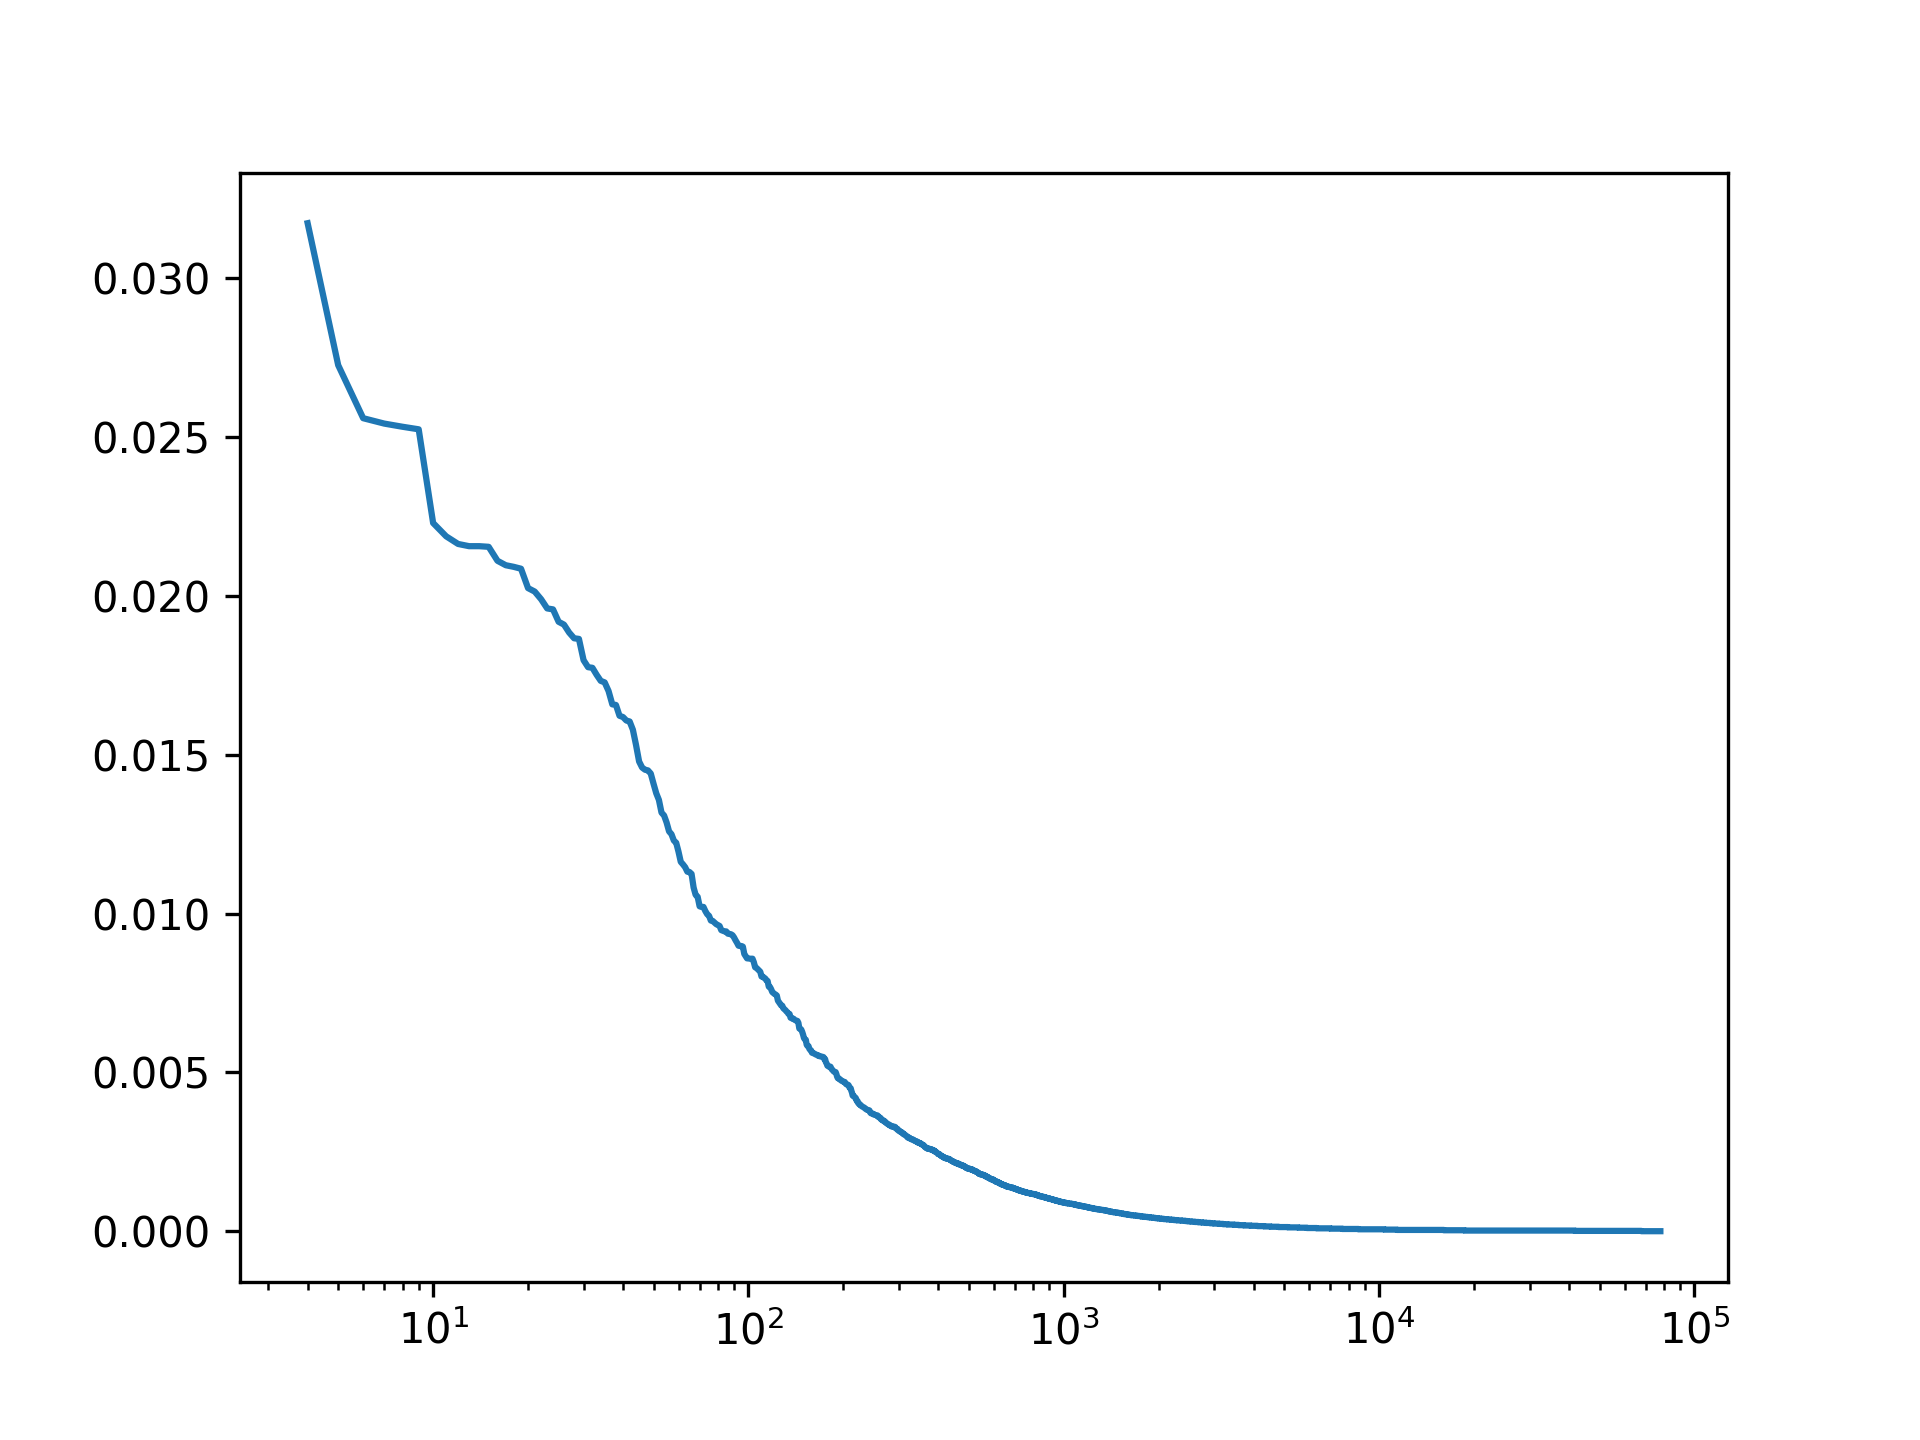
\includegraphics[width=130mm]{figures/unigrams.png}
\caption{Mutual information of unigrams}\label{fig:mi_unigrams}
\end{figure}


\begin{figure}[ht]\centering
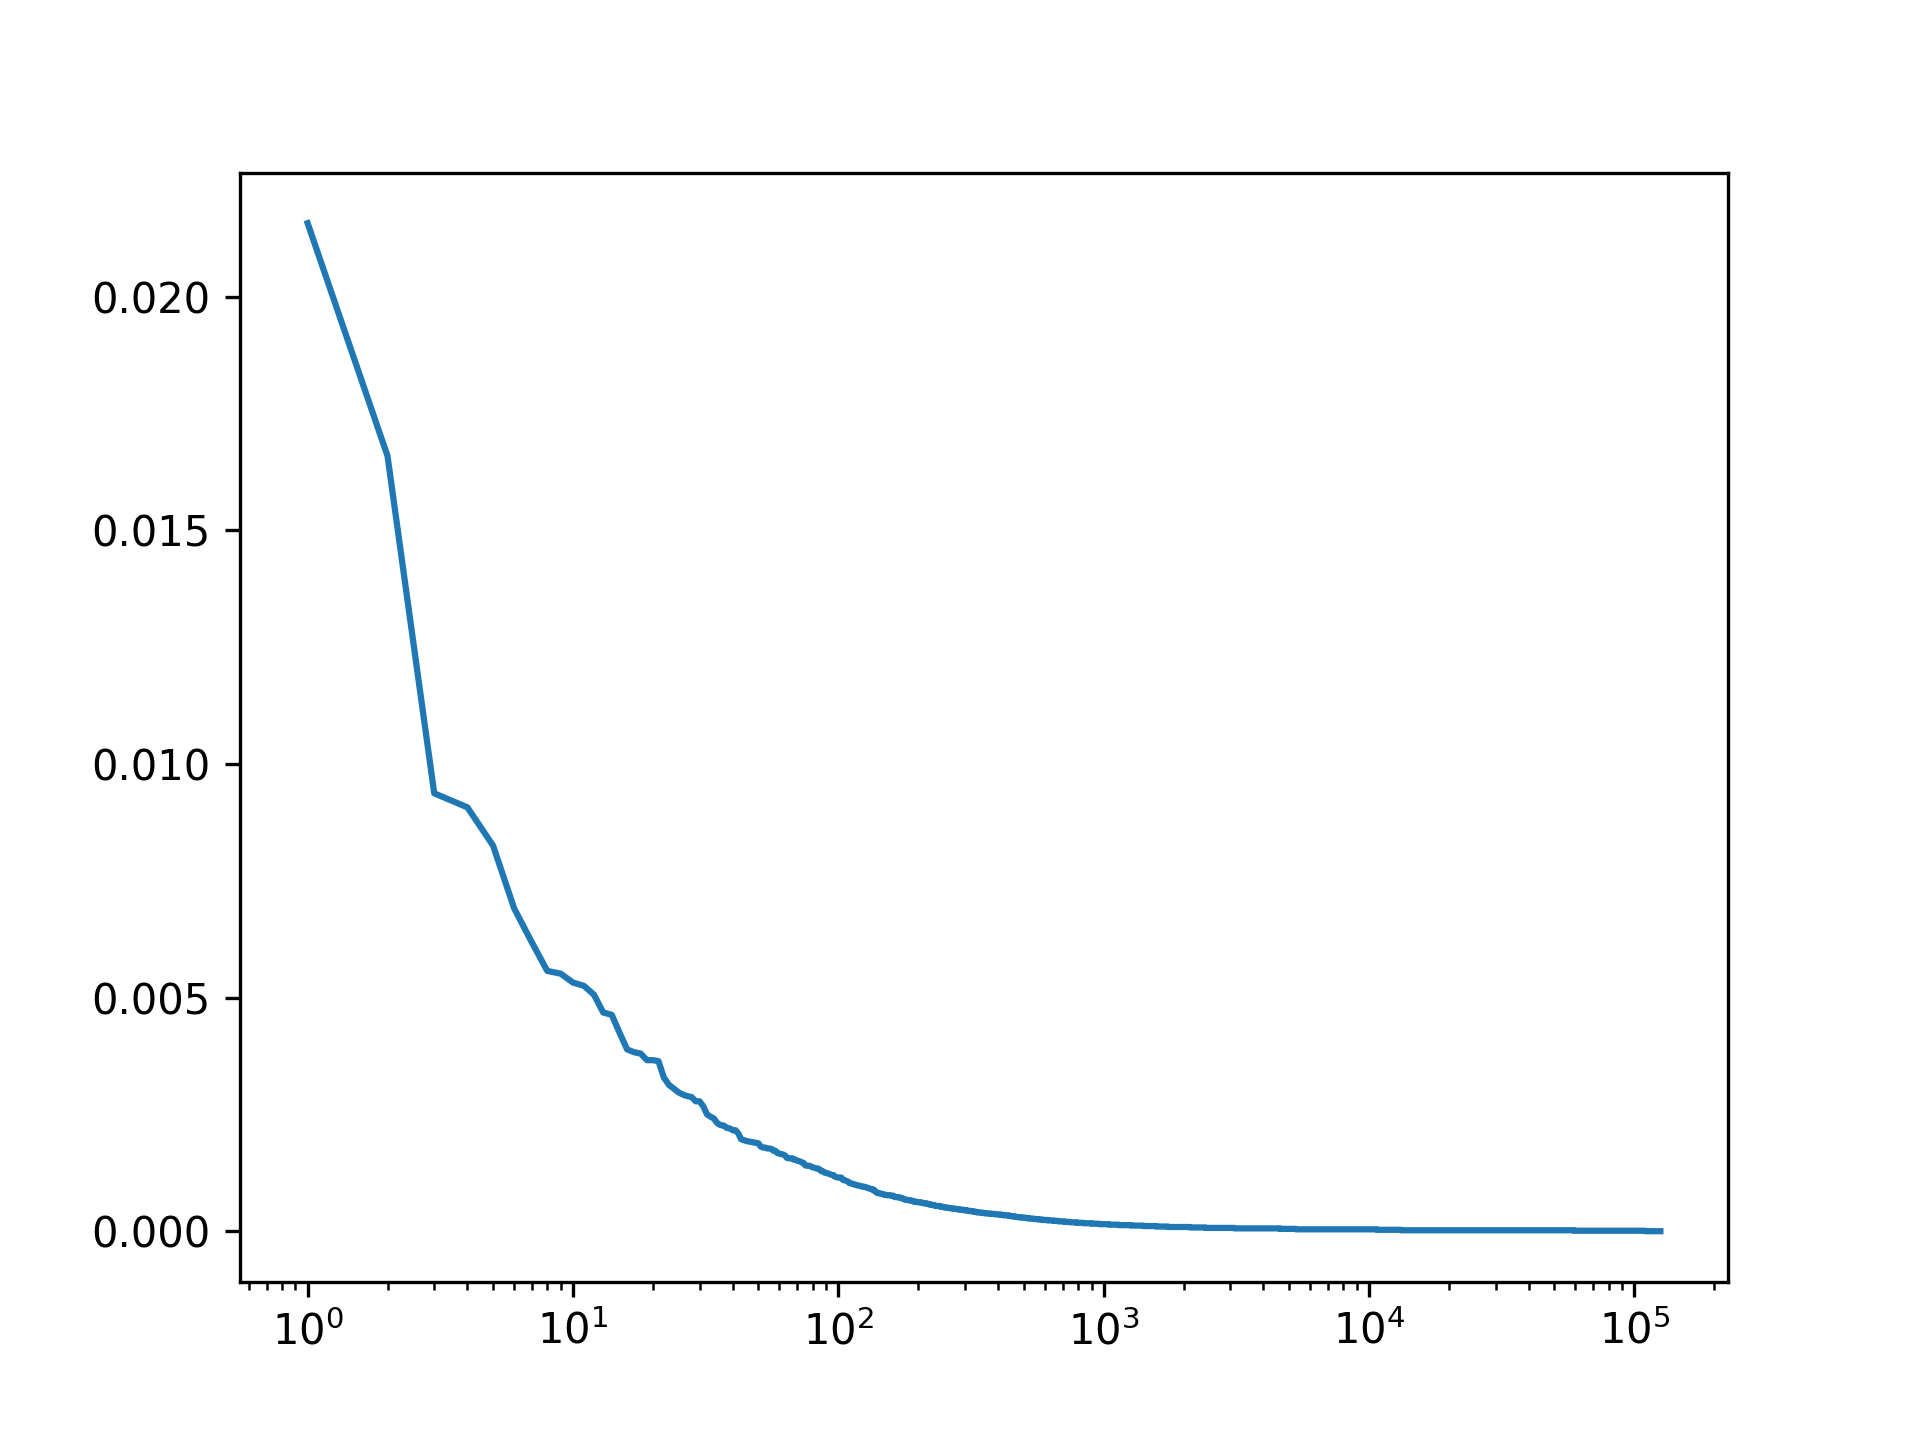
\includegraphics[width=130mm]{figures/entities.png}
\caption{Mutual information of entities}\label{fig:mi_entities}
\end{figure}


In this chapter, we described the exact process of building dataset,
reported basic statistics along with mutual information of extracted features.
In the next chapter, we discuss the results of experiments.
